

\documentclass[border=5pt]{standalone}
\usepackage[dvipsnames]{xcolor}
\usepackage{tikz}
\usepackage{pgfmath}
\usetikzlibrary{decorations.text, arrows.meta,calc,shadows.blur,shadings}
% arctext from Andrew code with modifications:
%Variables: 1: ID, 2:Style 3:box height 4: Radious 5:start-angl 6:end-angl 7:text {format along path} 
\def\arctext[#1][#2][#3](#4)(#5)(#6)#7{
    \draw[#2] (#5:#4cm+#3) coordinate (above #1) arc (#5:#6:#4cm+#3) 
    -- (#6-5:#4) coordinate (right #1) -- (#6:#4cm-#3) coordinate (below right #1) arc (#6:#5:#4cm-#3) coordinate (below #1)
    -- (#5-5:#4) coordinate (left #1) -- cycle;
    \path[
    decoration={
        raise = -0.5ex, % Controls relavite text height position.
        text  along path,
        text = {#7},
        text align = center,        
    },
    decorate
    ]
    (#5-5:#4) arc (#5-5:#6:#4);
}

\begin{document}
    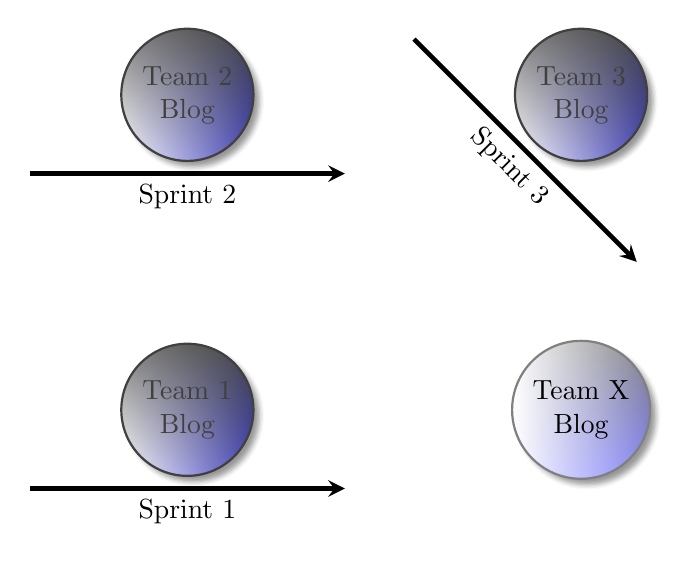
\begin{tikzpicture}[
        % Styles
        ShdShape/.style ={
            color=#1!50!black,
            thick,
            upper left=#1,
            upper right=black!50!#1,
            lower left=white,
            lower right=blue!50!#1,
            blur shadow, %Tikzedt not suport online view
        }
        ]           
        % you can anidate this in a new drawing definition
        \def\Sprint[#1](#2)[#3]#4#5#6#7#8{
            \begin{scope}[shift={(#1)},rotate=#2] 
                \node[ShdShape=gray,draw,align=center,circle](CENTER) at (0,0) {Team #3 \\ Blog};
                \arctext[SSN][ShdShape=orange][8pt](2)(25)(-20){|\footnotesize\color{black}|#8};
                \arctext[SCap][ShdShape=yellow][8pt](2)(75)(27){|\footnotesize\color{black}|#7};
                \arctext[SRel][ShdShape=lime][8pt](2)(107)(77){|\footnotesize\color{black}|#6};
                \arctext[SRel][ShdShape=green][8pt](2)(152)(109){|\footnotesize\color{black}|#5};
                \arctext[SRel][ShdShape=SeaGreen][8pt](2)(200)(154){|\footnotesize\color{black}|#4};
                \draw[-stealth, ultra thick](-2,-1)to node[below, midway,rotate=#2]{Sprint #3}++(4,0);
            \end{scope}
        }
        
        %Then draw many of these in other positions...  
        \Sprint[0,0](0)[1]{Design}{Develop}{Test}{Deploy}{Review}
        \Sprint[0,4](0)[2]{Task 1}{Task 2}{Task 3}{Task 4}{Task 5}
        \Sprint[5,4](-45)[3]{Task 6}{Task 7}{Task 8}{Task 9}{too much...}
        
        %Or you can shift or rotate a part of new drawings using scope.
        \begin{scope}[shift={(5,0)},rotate=15] 
        \node[ShdShape=white,draw,align=center,circle,text=black](CENTER) at (0,0) {Team X \\ Blog};
        \arctext[SSN][ShdShape=blue!50!green][8pt](1)(180)(0){|\footnotesize\color{black}|personalized};
        \arctext[SCap][ShdShape=cyan][8pt](1)(180)(360){|\footnotesize\color{black}|option};
        \end{scope}
\end{tikzpicture}
    
\end{document}